% Manuel de SudokuSolver (fr). Compilation : python3 docs/src/compiler.py
% Préambule commun aux manuels de SudokuSolver (français et anglais), au
% format maison des PDF : Latin Modern, titres sans-serif colorés (sky pour
% les sections, alert pour les sous-sections), encadrés tcolorbox, icônes
% fontawesome, anti-titres orphelins, page de garde avec le logo.
% Compilation : python3 docs/src/compiler.py (depuis la racine du dépôt).
\documentclass[11pt,a4paper]{article}
\usepackage[utf8]{inputenc}
\usepackage[T1]{fontenc}
\usepackage{lmodern}
\usepackage{microtype}
\usepackage[a4paper,margin=2cm,headheight=24pt]{geometry}
\usepackage{graphicx}
\usepackage[table]{xcolor}
\usepackage[most]{tcolorbox}
\usepackage{enumitem}
\usepackage{booktabs}
\usepackage{array}
\usepackage{tabularx}
\usepackage[nobottomtitles*]{titlesec}
\usepackage{needspace}
\usepackage{fancyhdr}
\usepackage{fontawesome5}
\usepackage{etoolbox}
\usepackage{listings}
\usepackage{amssymb}
\usepackage[colorlinks=true,linkcolor=sky,urlcolor=sky]{hyperref}
\graphicspath{{../captures/}{../../}}
\input{version}

\definecolor{sky}{HTML}{1C6DB4}
\definecolor{skyl}{HTML}{E6F0F9}
\definecolor{alert}{HTML}{B5382B}
\definecolor{alertl}{HTML}{FBEAE8}
\definecolor{steppe}{HTML}{C08A2E}
\definecolor{steppel}{HTML}{FBF1DC}
\definecolor{summit}{HTML}{6B7A8F}
\definecolor{night}{HTML}{232A56}
\definecolor{ink}{HTML}{1F2430}
\definecolor{codegray}{HTML}{2B2B2B}
\AtBeginDocument{\color{ink}}
% Noms de couleurs de l'ancien manuel, ramenés à la palette maison
\colorlet{darkblue}{night}
\colorlet{midblue}{sky}
\colorlet{lightblue}{skyl}
\colorlet{accent}{steppe}
\definecolor{success}{HTML}{2E7D5B}
\colorlet{danger}{alert}
\definecolor{softgray}{HTML}{F6F6F6}

\titleformat{\section}
  {\Large\bfseries\sffamily\color{sky}}
  {\thesection}{0.6em}{}
  [{\vspace{1pt}\color{sky!35}\titlerule[1.3pt]}]
\titlespacing*{\section}{0pt}{16pt}{8pt}
\titleformat{\subsection}{\large\bfseries\sffamily\color{alert}}{\thesubsection}{0.5em}{}
\titlespacing*{\subsection}{0pt}{12pt}{4pt}
\titleformat{\subsubsection}{\normalsize\bfseries\sffamily\color{night}}{\thesubsubsection}{0.5em}{}
\pretocmd{\section}{\needspace{12\baselineskip}}{}{}
\pretocmd{\subsection}{\needspace{6\baselineskip}}{}{}
\widowpenalty=10000
\clubpenalty=10000
\raggedbottom
\setlength{\parindent}{0pt}
\setlength{\parskip}{6pt}
\setlist{topsep=3pt,itemsep=2pt}

\pagestyle{fancy}
\fancyhf{}
\renewcommand{\headrulewidth}{0.4pt}
\renewcommand{\headrule}{\hbox to\headwidth{\color{sky!40}\leaders\hrule height \headrulewidth\hfill}}
\fancyhead[L]{\sffamily\small\color{sky}\textbf{SudokuSolver} \color{summit}\textbar{} \MANUELTITRE}
\fancyhead[R]{\sffamily\small\color{summit}\thepage}
\fancyfoot[C]{\sffamily\scriptsize\color{summit}Version \VERSIONAPP{} \textbar{} github.com/ARP273-ROSE/SudokuSolver}

\newcommand{\menu}[1]{\textsf{\textbf{\textcolor{sky}{#1}}}}
\newcommand{\touche}[1]{\tcbox[on line,boxsep=0pt,left=2pt,right=2pt,top=1.5pt,bottom=1.5pt,
  colback=white,colframe=summit,boxrule=0.5pt,arc=1.5pt]{\footnotesize\textsf{#1}}}
\newcommand{\fichier}[1]{\texttt{\small #1}}
\newcommand{\capture}[2][1]{\par\needspace{12\baselineskip}\begin{center}\setlength{\fboxsep}{0pt}\setlength{\fboxrule}{0.6pt}%
  \fcolorbox{summit!50}{white}{\includegraphics[width=\dimexpr#1\linewidth-1.3pt\relax]{#2}}\end{center}}

% Deux captures côte à côte, chacune avec sa légende, jamais séparées
\newcommand{\deuxcaptures}[4]{\par\needspace{22\baselineskip}\begin{center}\setlength{\fboxsep}{0pt}\setlength{\fboxrule}{0.6pt}%
  \begin{minipage}[t]{0.47\linewidth}\centering\fcolorbox{summit!50}{white}{\includegraphics[width=\dimexpr\linewidth-1.3pt\relax]{#1}}\\[3pt]{\small\sffamily\color{summit}#2}\end{minipage}\hfill
  \begin{minipage}[t]{0.47\linewidth}\centering\fcolorbox{summit!50}{white}{\includegraphics[width=\dimexpr\linewidth-1.3pt\relax]{#3}}\\[3pt]{\small\sffamily\color{summit}#4}\end{minipage}\end{center}}

% Encadrés (mêmes noms et signatures que l'ancien manuel)
\newtcolorbox{infobox}[1][]{enhanced,unbreakable,colback=skyl,colframe=sky,boxrule=0.9pt,arc=2.5pt,
  left=2.5mm,right=2.5mm,top=1.5mm,bottom=1.5mm,borderline west={2.5pt}{-2.5pt}{sky},#1}
\newtcolorbox{tipbox}[2][]{enhanced,unbreakable,colback=steppel,colframe=steppe!85!black,
  coltitle=white,fonttitle=\bfseries\sffamily\small,boxrule=0.9pt,arc=2.5pt,
  left=2.5mm,right=2.5mm,top=1.5mm,bottom=1.5mm,title={\faLightbulb~~#2},#1}
\newtcolorbox{warnbox}[2][]{enhanced,unbreakable,colback=alertl,colframe=alert,
  coltitle=white,fonttitle=\bfseries\sffamily\small,boxrule=0.9pt,arc=2.5pt,
  left=2.5mm,right=2.5mm,top=1.5mm,bottom=1.5mm,title={\faExclamationTriangle~~#2},#1}

\lstset{basicstyle=\ttfamily\small\color{white},backgroundcolor=\color{codegray},
  frame=single,framerule=0pt,rulecolor=\color{codegray},xleftmargin=6pt,xrightmargin=6pt,
  framexleftmargin=6pt,framexrightmargin=6pt,aboveskip=6pt,belowskip=6pt,
  breaklines=true,showstringspaces=false,
  literate={é}{{\'e}}1 {è}{{\`e}}1 {à}{{\`a}}1 {ê}{{\^e}}1 {ç}{{\c c}}1}

\newcommand{\pagedegarde}[2]{%
  \begin{titlepage}
  \thispagestyle{empty}
  \vspace*{1.4cm}
  \begin{center}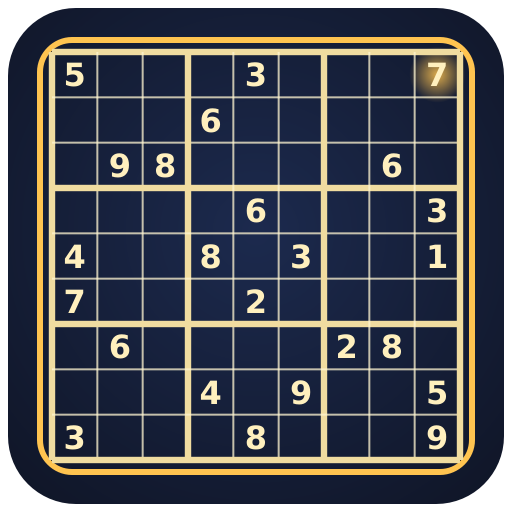
\includegraphics[width=4.4cm]{logo_512.png}\end{center}
  \vspace{8mm}
  {\sffamily\color{summit}\large SudokuSolver\par}
  \vspace{4mm}
  {\color{sky!35}\hrule height 2pt}
  \vspace{7mm}
  {\sffamily\bfseries\color{sky}\fontsize{26}{30}\selectfont #1\par}
  \vspace{4mm}
  {\sffamily\color{night}\large #2\par}
  \vspace{7mm}
  {\color{sky!35}\hrule height 2pt}
  \vspace{5mm}
  {\sffamily\color{summit}\normalsize Version \VERSIONAPP\par}
  \vfill
  {\sffamily\small\color{summit} MIT \textbar{} github.com/ARP273-ROSE/SudokuSolver\par}
  \end{titlepage}}

\usepackage[french]{babel}
\newcommand{\MANUELTITRE}{Manuel d'utilisation}
\begin{document}
\pagedegarde{Manuel d'utilisation}{Solveur, générateur et tuteur de sudoku bilingue}
\tableofcontents
\newpage
% =================================================================
\section{Présentation}
% =================================================================

SudokuSolver est une application de bureau qui résout, génère et
enseigne les grilles de Sudoku. Écrite en Python avec une interface
graphique PyQt6, elle fonctionne sous Windows, Linux et macOS.
L'interface est entièrement bilingue (français / anglais) et chaque
contrôle dispose d'une infobulle dans les deux langues.

\begin{infobox}
\textbf{Fonctionnalités clés}
\begin{itemize}
  \item Solveur rapide : propagation de contraintes par masques binaires et backtracking MRV
  \item 8 techniques humaines avec explications pas-à-pas
  \item Générateur 4 niveaux, calibré par nombre d'indices et technique maximale requise
  \item Grille interactive 9$\times$9, candidats, détection d'erreurs en temps réel
  \item Multiplateforme (Windows, Linux, macOS)
  \item Rapports de crash automatiquement anonymisés (pas de nom d'utilisateur ni de chemin)
\end{itemize}
\end{infobox}

% =================================================================
\section{Installation}\label{sec:fr-install}
% =================================================================

\subsection{L'installeur (recommandé)}

Les paquets prêts à l'emploi, Python compris, sont publiés sur la
\href{https://github.com/ARP273-ROSE/SudokuSolver/releases/latest}{page des versions}.
Aucun droit d'administrateur n'est demandé : tout s'installe dans votre profil.

\begin{center}
\begin{tabularx}{\linewidth}{@{}l>{\raggedright\arraybackslash}X@{}}
\toprule
\textbf{Système} & \textbf{Fichier et premier lancement} \\
\midrule
Windows & \fichier{SudokuSolver-Setup.exe}. Si SmartScreen prévient que
l'installeur n'est pas signé : \emph{Informations complémentaires}, puis
\emph{Exécuter quand même} (une seule fois). \\
macOS & \fichier{SudokuSolver-X.Y.Z-macos-arm64.dmg} (Apple Silicon) ou
\fichier{-macos-x86\_64.dmg} (Intel) : glisser l'application dans
Applications, puis la première fois \emph{clic droit > Ouvrir}. \\
Linux & \fichier{SudokuSolver-X.Y.Z-linux-x86\_64.tar.gz} (ou
\fichier{-linux-arm64}) : décompresser, puis lancer \fichier{./installer.sh}
(installation dans \fichier{\textasciitilde/.local/share}, entrée de menu, sans sudo). \\
\bottomrule
\end{tabularx}
\end{center}

Cette adresse pointe toujours vers le dernier installeur Windows :
\begin{center}\footnotesize\url{https://github.com/ARP273-ROSE/SudokuSolver/releases/latest/download/SudokuSolver-Setup.exe}\end{center}

\subsection{Mises à jour}

Une fois installé, SudokuSolver cherche une nouvelle version au démarrage et
sur demande (\menu{Aide > Rechercher des mises à jour}). Il ne télécharge que
la petite archive applicative depuis GitHub (toute autre adresse est
refusée), la pose et redémarre --- sous Windows, macOS et Linux. Les notes
de version s'affichent dans la langue de l'interface.

\subsection{Rapports de problème}

Au premier lancement, SudokuSolver demande s'il peut envoyer automatiquement
un court rapport technique en cas de plantage ou de gel (version, système,
trace de l'erreur ; rien d'autre). Ce choix se modifie à tout moment dans le
menu \menu{Aide}, où \menu{Signaler un problème\dots} permet aussi d'écrire
soi-même un signalement.

\subsection{Depuis les sources}

Prérequis : Python 3.10 ou plus récent, \texttt{PyQt6} $\geq$ 6.5.
Sous Windows, \fichier{launch.bat} détecte Python, crée un environnement
virtuel dans \fichier{\%APPDATA\%\textbackslash SudokuSolver\textbackslash venv}
et lance l'application ; \fichier{launch.bat --repair} le reconstruit.
Sous Linux et macOS, \fichier{./launch.sh} fait de même dans
\fichier{\$XDG\_DATA\_HOME/SudokuSolver/venv}. À la main :

\begin{lstlisting}
pip install -r requirements.txt
python main.py
\end{lstlisting}

% =================================================================
\section{L'interface}
% =================================================================

\subsection{Fenêtre principale}

La fenêtre comporte quatre zones principales~:

\begin{enumerate}
  \item \textbf{Barre supérieure} --- sélecteur de difficulté et bouton ``Nouvelle grille''.
  \item \textbf{Grille} --- le plateau 9$\times$9 interactif.
  \item \textbf{Barre d'actions} --- Indice, Étape suivante, Résoudre, Vérifier, Candidats, Réinitialiser.
  \item \textbf{Zone d'explication} et \textbf{barre d'état} en bas.
\end{enumerate}

\deuxcaptures{fr-principal.png}{La fenêtre principale, avec les candidats}{fr-indice.png}{Un indice : la case en vert, l'explication en dessous}

\subsection{Clavier}

\begin{center}
\begin{tabular}{>{\bfseries\color{darkblue}}l l}
\rowcolor{lightblue}
Touche & Action \\
\hline
Flèches              & Déplacer la sélection \\
\rowcolor{softgray}
1--9                 & Saisir un chiffre dans la case courante \\
0, Suppr, Retour arr.& Effacer la case \\
\rowcolor{softgray}
Clic souris          & Sélectionner une case \\
\end{tabular}
\end{center}

\subsection{États d'une case}

\begin{itemize}
  \item \textbf{Donnée} --- indice original, non modifiable, affiché en gras.
  \item \textbf{Saisie utilisateur} --- chiffre que vous avez tapé, dans une couleur distincte.
  \item \textbf{Conflit} --- le contenu enfreint une règle ligne, colonne ou bloc ; le fond devient rouge.
  \item \textbf{Candidats} --- petits chiffres montrant les valeurs possibles, activés par le bouton ``Candidats''.
\end{itemize}

% =================================================================
\section{Fonctionnalités}
% =================================================================

\subsection{Générer une grille}

Choisissez une difficulté dans la liste déroulante et cliquez sur
\textbf{Nouvelle grille}. Le générateur crée une grille avec symétrie
rotationnelle, solution unique garantie, et calibre le nombre d'indices
et la technique la plus difficile requise pour correspondre à la
difficulté cible.

\begin{center}
\begin{tabular}{>{\color{darkblue}\bfseries}l c c}
\rowcolor{lightblue}
Niveau     & Indices & Technique maximale \\
\hline
Facile     & 36--45 & Singleton caché \\
\rowcolor{softgray}
Moyen      & 30--35 & Paire cachée \\
Difficile  & 26--32 & Réduction bloc / ligne \\
\rowcolor{softgray}
Expert     & 22--28 & X-Wing \\
\end{tabular}
\end{center}

La génération s'exécute dans un thread d'arrière-plan, l'interface ne
gèle jamais, même si le générateur doit réessayer plusieurs fois pour
atteindre la difficulté cible.

\subsection{Indice}

Cliquez sur \textbf{Indice} pour voir le prochain coup logique. Le
moteur choisit la technique applicable la plus simple, met en évidence
les cases du motif en vert et les candidats éliminés en rouge, puis
explique \emph{pourquoi} le coup fonctionne.

\begin{tipbox}{Astuce}
Si aucune technique ne s'applique, le moteur bascule sur une hypothèse
basée sur le solveur par backtracking. C'est très rare pour les grilles
générées, mais peut arriver sur des grilles importées nécessitant des
techniques avancées non encore implémentées.
\end{tipbox}

\subsection{Étape suivante}

Comme Indice, mais \emph{applique} l'étape automatiquement. Enchaînez
plusieurs clics ``Étape suivante'' pour regarder la grille se résoudre
technique par technique.

\subsection{Résoudre}

Remplit la solution complète instantanément. Le solveur rapide
s'exécute dans un thread d'arrière-plan et est plafonné à 2\,000\,000
de n\oe uds de recherche, ce qui garantit l'absence de gel même sur des
entrées pathologiques.

\subsection{Vérifier}

Compare chaque chiffre saisi par l'utilisateur à la solution stockée.
Les cases incorrectes sont surlignées en rouge, les cases correctes en
vert. Utile quand vous n'êtes pas sûr qu'une déduction était valide.

\subsection{Candidats}

Active ou désactive l'affichage des candidats. Activé, chaque case vide
affiche son ensemble courant de candidats en petits chiffres. Désactivé,
les cases restent propres --- utile pour une vue moins chargée quand
vous êtes confiant sur une région.

\subsection{Réinitialiser}

Efface toutes les saisies utilisateur et restaure la grille dans son
état généré. Les indices originaux sont préservés.

\subsection{Menu Fichier}

\begin{itemize}
  \item \textbf{Nouvelle} --- génère une nouvelle grille à la difficulté courante.
  \item \textbf{Ouvrir} --- charge une chaîne de 81 caractères depuis un fichier
        \texttt{.txt} ou \texttt{.sdk}. Taille du fichier plafonnée à 10\,Ko.
  \item \textbf{Enregistrer} --- sauvegarde la grille courante sous forme de chaîne
        de 81 caractères (points pour les cases vides).
  \item \textbf{Quitter} --- ferme l'application.
\end{itemize}

\subsection{Menu Langue}

Bascule toute l'interface entre français et anglais, immédiatement. Au
premier lancement, la langue est celle du système ; le choix fait ici est
retenu.

\subsection{Menu Aide}

\begin{itemize}
  \item \textbf{Manuel (PDF)} --- ce document, dans la langue de l'interface (\touche{F1}).
  \item \textbf{Comment jouer} --- un court guide intégré.
  \item \textbf{Techniques de résolution} --- un catalogue bilingue complet des
        8 techniques implémentées (voir aussi \fichier{guide\_techniques.pdf}).
  \item \textbf{Rechercher des mises à jour} --- voir la section~\ref{sec:fr-install}.
  \item \textbf{Signaler un problème\dots} --- écrire un signalement, transmis avec l'état de la grille.
  \item \textbf{Envoyer automatiquement les rapports de problème} --- l'accord demandé au premier lancement.
  \item \textbf{À propos} --- version et crédits.
\end{itemize}

% =================================================================
\section{Sous le capot}
% =================================================================

\subsection{Architecture du solveur}

Le solveur représente les ensembles de candidats sous forme de masques
9 bits (\texttt{1<<(d-1)} pour le chiffre \texttt{d}). Chaque case
connaît l'intersection bit à bit des chiffres autorisés pour sa ligne,
sa colonne et son bloc. Placer un chiffre met à jour les masques de
candidats des pairs en temps constant.

La recherche utilise l'heuristique MRV (\emph{Minimum Remaining
Values}) : choisir la case vide avec le moins de candidats, essayer
chaque candidat, propager, récurser. C'est le schéma utilisé par le
célèbre solveur de Peter Norvig, étendu avec un plafond explicite de
n\oe uds qui borne l'effort dans le pire cas.

\subsection{Techniques humaines}

Le solveur humain implémente huit techniques, essayées par ordre de
difficulté croissante~:

\begin{center}
\begin{tabular}{>{\color{darkblue}\bfseries}l l}
\rowcolor{lightblue}
Technique & Ce qu'elle détecte \\
\hline
Singleton nu        & Case n'ayant plus qu'un candidat \\
\rowcolor{softgray}
Singleton caché     & Chiffre ne pouvant tenir que dans une case d'une unité \\
Paire nue           & Deux cases partageant exactement deux candidats \\
\rowcolor{softgray}
Triplet nu          & Trois cases partageant trois candidats \\
Paire cachée        & Deux chiffres ne pouvant tenir que dans les deux mêmes cases \\
\rowcolor{softgray}
Paire pointante     & Candidats d'un bloc alignés sur une même ligne ou colonne \\
Réduction bloc/ligne& Candidats d'une ligne confinés à un seul bloc \\
\rowcolor{softgray}
X-Wing              & Motif d'élimination rectangulaire 2$\times$2 \\
\end{tabular}
\end{center}

Voir \texttt{guide\_techniques.pdf} pour des exemples détaillés de
chaque technique.

\subsection{Générateur}

La génération part d'une solution valide aléatoire (backtracking
mélangé), puis retire les indices de façon symétrique en vérifiant après
chaque retrait que la grille conserve exactement une solution. Le
résultat est évalué en comptant les indices et en faisant tourner le
solveur humain pour identifier la technique la plus difficile requise.
Si l'évaluation ne correspond pas à la difficulté cible, la génération
réessaie jusqu'à 40 fois avant de se rabattre sur la correspondance la
plus proche.

\subsection{Threads et anti-gel}

Tout le travail long (génération, résolution) s'exécute dans des
\texttt{QThread} dédiés. Le thread de l'interface reste réactif et la
fenêtre ne gèle jamais, même si vous cliquez plusieurs fois d'affilée
sur ``Nouvelle grille'' ou importez une grille pathologiquement
difficile.

Le cycle de vie des workers est géré de façon défensive : quand un
thread se termine, son wrapper Python est vidé \emph{avant} que l'objet
natif Qt ne soit détruit, de sorte que les opérations suivantes ne
touchent jamais une référence pendante.

\subsection{Rapports de crash}

Les exceptions non rattrapées sont interceptées par un \texttt{sys.excepthook}
qui écrit un rapport JSON anonymisé (trace, versions, système --- jamais le
nom d'utilisateur ni le dossier personnel) dans le dossier de données et,
avec votre accord, le transmet au point de collecte, comme les plantages
natifs et les gels de l'interface (une vigie remarque quand la fenêtre ne
répond plus). Le dossier de données est hors du dossier d'installation, que
les mises à jour remplacent :
\fichier{\%LOCALAPPDATA\%\textbackslash SudokuSolver} sous Windows,
\fichier{\textasciitilde/Library/Application Support/SudokuSolver} sous macOS,
\fichier{\textasciitilde/.local/share/SudokuSolver} sous Linux.

% =================================================================
\section{Dépannage}
% =================================================================

\subsection{``Python not found'' sous Windows}

Le launcher n'a pas trouvé d'interpréteur Python fonctionnel. Installez
Python 3.10 ou plus récent depuis
\url{https://www.python.org/downloads/} et \textbf{cochez bien
``Add Python to PATH''} pendant l'installation. Puis relancez
\texttt{launch.bat}.

\subsection{``Installation failed'' après une mise à jour de Python}

Si vous avez mis à jour Python et que l'ancien venv est obsolète,
exécutez~:

\begin{lstlisting}
launch.bat --repair
\end{lstlisting}

Cela supprime l'environnement virtuel et réinstalle tout proprement.

\subsection{Le générateur est lent en Expert}

Les grilles Expert qui nécessitent spécifiquement un X-Wing sont rares,
donc le générateur peut réessayer jusqu'à 40 fois avant de se rabattre
sur une grille Difficile avec un nombre d'indices légèrement plus
contraint. C'est intentionnel, et le thread d'arrière-plan garde
l'interface réactive pendant toute l'opération.

\subsection{J'ai importé une grille et Résoudre dit ``pas de solution''}

Soit la grille importée contient une erreur de saisie (mauvais chiffre
dans un indice), soit elle contient déjà un conflit (vérifiez les cases
rouges), soit elle n'a réellement pas de solution. Le solveur abandonne
aussi après 2\,000\,000 de n\oe uds de recherche --- cela ne se
déclenche presque jamais sur une grille 9$\times$9 valide.

\subsection{Où sont stockés mes réglages ?}

Le seul réglage, la langue, est conservé par Qt dans les préférences de
l'utilisateur (registre sous Windows, \fichier{\textasciitilde/.config} sous
Linux, préférences sous macOS). Le journal et les rapports vivent dans le
dossier de données décrit à la section \emph{Rapports de crash} ; rien n'est
écrit dans le dossier d'installation.

\subsection{L'application a planté --- que faire ?}

Si vous avez accepté l'envoi automatique, il n'y a rien à faire : le rapport
est parti. Sinon, passez par \menu{Aide > Signaler un problème\dots} et
décrivez ce que vous faisiez ; sans connexion, le rapport est enregistré en
\fichier{.zip} sur le Bureau, prêt à joindre à un ticket GitHub.

% =================================================================
\section{FAQ}
% =================================================================

\subsubsection*{Puis-je jouer sur téléphone ?}
Non --- c'est une application de bureau. Pour le mobile, utilisez une
application Sudoku dédiée sur le store de votre plateforme.

\subsubsection*{Y a-t-il de la télémétrie ?}
Seulement pour deux choses : la recherche de mise à jour (API des versions
de GitHub, une fois au démarrage) et, si vous l'avez accepté, les rapports de
problème. Aucune statistique, aucune grille transmise sauf dans un
signalement écrit.

\subsubsection*{Quels formats de Sudoku sont pris en charge ?}
Les chaînes de 81 caractères avec chiffres \texttt{1--9} et l'un de
\texttt{.}, \texttt{0}, \texttt{-} ou espace pour les cases vides. Les
retours à la ligne sont tolérés.

\subsubsection*{Pourquoi le guide des techniques est-il un PDF séparé ?}
Parce que c'est une référence que vous voudrez consulter pendant la
résolution. Le manuel principal (ce document) est le guide
``comment utiliser l'application'' ; le guide des techniques est la
référence ``comment résoudre un Sudoku''.

% =================================================================
\section{Crédits}
% =================================================================

SudokuSolver est distribué sous licence MIT. Merci à Peter Norvig pour
le schéma classique du solveur par propagation de contraintes, et à la
communauté Sudoku pour des décennies de catalogue de techniques
accumulées.

\medskip
Les tickets et contributions sont les bienvenus sur~:\\
\url{https://github.com/ARP273-ROSE/SudokuSolver}

\vfill
\begin{center}
\color{midblue}\small
SudokuSolver --- Manuel utilisateur --- v1.1.1
\end{center}
\end{document}
